% Masters/Doctoral Thesis 
% LaTeX Template
% Version 2.5 (27/8/17)
%
% This template was downloaded from:
% http://www.LaTeXTemplates.com
%
% Version 2.x major modifications by:
% Vel (vel@latextemplates.com)
%
% This template is based on a template by:
% Steve Gunn (http://users.ecs.soton.ac.uk/srg/softwaretools/document/templates/)
% Sunil Patel (http://www.sunilpatel.co.uk/thesis-template/)
%
% Template license:
% CC BY-NC-SA 3.0 (http://creativecommons.org/licenses/by-nc-sa/3.0/)
%
%%%%%%%%%%%%%%%%%%%%%%%%%%%%%%%%%%%%%%%%%

%----------------------------------------------------------------------------------------
%	PACKAGES AND OTHER DOCUMENT CONFIGURATIONS
%----------------------------------------------------------------------------------------

\documentclass[
11pt, % The default document font size, options: 10pt, 11pt, 12pt
%oneside, % Two side (alternating margins) for binding by default, uncomment to switch to one side
english, % ngerman for German
singlespacing, % Single line spacing, alternatives: onehalfspacing or doublespacing
%draft, % Uncomment to enable draft mode (no pictures, no links, overfull hboxes indicated)
%nolistspacing, % If the document is onehalfspacing or doublespacing, uncomment this to set spacing in lists to single
liststotoc, % Uncomment to add the list of figures/tables/etc to the table of contents
%toctotoc, % Uncomment to add the main table of contents to the table of contents
parskip, % Uncomment to add space between paragraphs
%nohyperref, % Uncomment to not load the hyperref package
%headsepline, % Uncomment to get a line under the header
%chapterinoneline, % Uncomment to place the chapter title next to the number on one line
consistentlayout, % Uncomment to change the layout of the declaration, abstract and acknowledgements pages to match the default layout
]{Thesis} % The class file specifying the document structure

\usepackage[utf8]{inputenc} % Required for inputting international characters
\usepackage[T1]{fontenc} % Output font encoding for international characters

\usepackage{mathpazo} % Use the Palatino font by default

\usepackage{listings}

\usepackage{amsmath}

\usepackage[backend=bibtex,style=ieee,natbib=true]{biblatex} % Use the bibtex backend with the authoryear citation style (which resembles APA)

\addbibresource{bibliography.bib} % The filename of the bibliography

\usepackage[autostyle=true]{csquotes} % Required to generate language-dependent quotes in the bibliography

%----------------------------------------------------------------------------------------
%	MARGIN SETTINGS
%----------------------------------------------------------------------------------------

\geometry{
	paper=a4paper, % Change to letterpaper for US letter
	inner=2.5cm, % Inner margin
	outer=3.8cm, % Outer margin
	bindingoffset=.5cm, % Binding offset
	top=1.5cm, % Top margin
	bottom=1.5cm, % Bottom margin
	%showframe, % Uncomment to show how the type block is set on the page
}

%----------------------------------------------------------------------------------------
%	THESIS INFORMATION
%----------------------------------------------------------------------------------------

\thesistitle{Multi Label Music Classification} % Your thesis title, this is used in the title and abstract, print it elsewhere with \ttitle
\supervisor{Carmen Pelaez Moreno} % Your supervisor's name, this is used in the title page, print it elsewhere with \supname
\degree{Computer Science} % Your degree name, this is used in the title page and abstract, print it elsewhere with \degreename
\author{Benjamin Hernandez Garcia} % Your name, this is used in the title page and abstract, print it elsewhere with \authorname
\university{Universidad Carlos III} % Your university's name and URL, this is used in the title page and abstract, print it elsewhere with \univname
\department{Department or Computer Science} % Your department's name and URL, this is used in the title page and abstract, print it elsewhere with \deptname
\AtBeginDocument{
	\hypersetup{pdftitle=\ttitle}
	\hypersetup{pdfauthor=\authorname}
	\hypersetup{colorlinks=false}
}
\begin{document}

\frontmatter % Use roman page numbering style (i, ii, iii, iv...) for the pre-content pages

\pagestyle{plain} % Default to the plain heading style until the thesis style is called for the body content

%----------------------------------------------------------------------------------------
%	TITLE PAGE
%----------------------------------------------------------------------------------------

\begin{titlepage}
\begin{center}

\vspace*{.06\textheight}
{\scshape\LARGE \univname\par}\vspace{1.5cm} % University name
\textsc{\Large Bachelor Thesis}\\[0.5cm] % Thesis type

\HRule \\[0.4cm] % Horizontal line
{\huge \bfseries \ttitle\par}\vspace{0.4cm} % Thesis title
\HRule \\[1.5cm] % Horizontal line
 
\begin{minipage}[t]{0.4\textwidth}
\begin{flushleft} \large
\emph{Author:}\\
{\authorname} % Author name - remove the \href bracket to remove the link
\end{flushleft}
\end{minipage}
\begin{minipage}[t]{0.4\textwidth}
\begin{flushright} \large
\emph{Supervisor:} \\
{\supname} % Supervisor name - remove the \href bracket to remove the link  
\end{flushright}
\end{minipage}\\[3cm]

{\large \today}\\[4cm] % Date
%\includegraphics{Logo} % University/department logo - uncomment to place it
 
\vfill
\end{center}
\end{titlepage}


%----------------------------------------------------------------------------------------
%	ACKNOWLEDGEMENTS
%----------------------------------------------------------------------------------------

\begin{acknowledgements}
\addchaptertocentry{\acknowledgementname} % Add the acknowledgements to the table of contents
I would like to thank every person who has made possible I could achieve my goals and become the person that I am today, especially my family and friends that have supported me over the years with continuous encouragement and kindness.

Thanks to my tutor, Carmen, that always helped and guided me during the entire process of this thesis even though I got stuck along the way.

Lastly, I would like to thank the random people over the internet that made their resources publicly available so others could use and consume them with documents, libraries, guides and an endless source of information free to use.
\end{acknowledgements}

%----------------------------------------------------------------------------------------
%	ABSTRACT PAGE
%----------------------------------------------------------------------------------------

\begin{abstract}
\addchaptertocentry{\abstractname} % Add the abstract to the table of contents
This paper explains and details the decisions and approaches taken to build a Multi-Label Classifier using Artificial Neural Networks based on Deep Learning techniques and deep music features to establish and predict the genre/s of a given song. 

The proposed method is based on Machine Learning techniques focused on Artifical Neural Networks. These networks try to learn tasks by emulating the way the human brain works. This set of algorithms are reasonably new and provide a yet to explore tools in the Artificial Intelligence field.

This paper aims to explain and analyze the accuracy and results obtained and might be used as a baseline for further music-related projects relying on classification techniques, such as recommender systems or sentiment analysis that could be enriched with the results of this paper.
\end{abstract}


%----------------------------------------------------------------------------------------
%	LIST OF CONTENTS/FIGURES/TABLES PAGES
%----------------------------------------------------------------------------------------

\tableofcontents % Prints the main table of contents

\listoffigures % Prints the list of figures

\listoftables % Prints the list of tables

%----------------------------------------------------------------------------------------
%	ABBREVIATIONS
%----------------------------------------------------------------------------------------

\begin{abbreviations}{ll} % Include a list of abbreviations (a table of two columns)
\textbf{AI} & \textbf{A}rtificial \textbf{I}ntelligence\\
\textbf{ANN} & \textbf{A}rtificial \textbf{N}eural \textbf{N}etworks\\
\textbf{BM-MLL} & \textbf{B}ack\textbf{p}ropagation for \textbf{M}ulti\textbf{l}abel \textbf{L}earning\\
\textbf{BR} & \textbf{B}ayesian \textbf{R}egression \\
\textbf{CNN} & \textbf{C}onvolutional \textbf{N}eural \textbf{N}etwork\\
\textbf{DAG} & \textbf{D}irected \textbf{A}cyclic \textbf{G}raph\\
\textbf{DMLPP} & \textbf{D}ual \textbf{M}ulti\textbf{l}abel \textbf{P}airwise \textbf{P}erceptron\\
\textbf{GDPR} & \textbf{G}eneral \textbf{D}ata \textbf{P}rotection \textbf{R}egulation\\
\textbf{JSON} & \textbf{J}ava\textbf{S}cript \textbf{O}bject \textbf{N}otation\\
\textbf{LSTM} & \textbf{L}ong-\textbf{S}hort-\textbf{t}erm \textbf{M}emory\\
\textbf{MFCC} & \textbf{M}el \textbf{F}requency \textbf{C}epstral \textbf{C}effcients\\
\textbf{ML} & \textbf{M}achine \textbf{L}aerning\\
\textbf{MLP} & \textbf{M}ulti \textbf{L}ayer \textbf{P}erceptron\\
\textbf{ML-RBF} & \textbf{M}ulti \textbf{L}abel \textbf{R}adial \textbf{B}asis \textbf{F}unction\\
\textbf{MMP} & \textbf{M}ulti-label \textbf{M}ulti-class \textbf{P}erceptron\\
\textbf{RNN} & \textbf{R}ecurrent \textbf{N}eural \textbf{N}etwork\\
\textbf{SVM} & \textbf{S}upport \textbf{V}ector \textbf{M}achines\\

\end{abbreviations}



%----------------------------------------------------------------------------------------
%	THESIS CONTENT - CHAPTERS
%----------------------------------------------------------------------------------------

\mainmatter % Begin numeric (1,2,3...) page numbering

\pagestyle{thesis} % Return the page headers back to the "thesis" style

% Include the chapters of the thesis as separate files from the Chapters folder
% Uncomment the lines as you write the chapters

% Chapter 1

\chapter{Introduction}

\label{introduction}
The following thesis will expose and explain the design, techniques, and development done and achieved to create a Music Genre Classifier based on its deep features.

The thesis explores the connections that may appear between musical pieces when combined using Deep Learning approaches as Artificial Neural Networks.

This project consists of the following stages:

\begin{itemize}
    \item Prepare the development environment and programming stack.
    \item Preprocessing of the provided data for the ease of use.
    \item Building of the appropriate dataset selecting the desired features and contents.
    \item Create the Artificial Neural Network model and the needed tools associated with it.
    \item Train the proposed model
    \item Evaluate the results and re-iterate the process to improve model accuracy.
\end{itemize}
  
The next sections will deeply explain and expose the decisions taken during the process of meeting the proposed requirements.
\newpage
%----------------------------------------------------------------------------------------

\section{Motives}
The motives behind this thesis roots in combining music with Artificial Intelligence techniques.

Artificial Neural Networks are a relatively new tool in the Machine Learning field that allows prototyping and creating capable models of virtually any learning task a human can reproduce.

Music genre classification has always been an important topic for the people who enjoy it. Labeling songs according to some formal and style features allow humans to enjoy a certain range of music compositions that better matches their preferences. The music classification also opens the possibility of creating recommender systems that provide the user with a variety of new compositions that the user might enjoy based on the proximity of the bunches several categories fall into. On top of that labeling, music provides a way to connect individual pieces with feelings and moods so the user can experience those mentioned just by listening to the appropriate song that may arise that feeling in them.

Music is a really powerful tool and a great expression of art that brings society together that must not be left unattended.

Combining these two distinctive facets is a considerable feat not to be interesting enough to left without exploring.

The author in this thesis is deeply interested in finding these connections previously mentioned and with the appropriate knowledge in both fields described to achieve the established goals.
\newpage
%----------------------------------------------------------------------------------------

\section{Objectives}
This thesis aims to create a classifier that labels songs with one or more genres looking for the best accuracy when facing new pieces. The project finds to create a model capable of properly labeling songs using its deep features rather than the song itself and establish a mathematical connection between the compositions and the genre or genres it may contain.

Artificial Neural Networks are a trendy topic that has been using for classification duties quite recently with still several aspects yet to be untwined and discovered

This project may serve itself as a complete activity with the achieved conclusions or as a preliminary base for future projects using the outcome obtained in the mentioned thesis.

\newpage
%----------------------------------------------------------------------------------------
\section{Legal Framework}

% TODO

\section{Socio-economic environment}
\subsection{Budget}

This thesis is meant to be completed within 4 months and 12 ECTS worth. 
According to the 'European Credit Transfer and Accumulation System \cite{ects}', a credit constitutes about 25 to 30 student hours which means 12 ECTS * 30 hours = 360 plus a 10\% of possible overload, would sum up roughly 400 hours of student time.

Including 1h weekly meetings with the supervisor during 19 weeks, this adds up to 19 hours plus a 6hours margin gives a total of 25 hours.

\begin{table}[h!]
    \centering
    \begin{tabular}{c c c c} 
        \hline
        Labour & Cost per hour & Total hours & Total \\ [0.5ex] 
        \hline
        Student & 12 & 400 & 4800 \\ 
        Supervisor & 20 & 25 & 500 \\
        \hline
        & & Sum & 5300 \\
        \hline
    \end{tabular}
    \caption{Human Resoures summary}
    \label{table:1}
\end{table}

Given all the software used is open-source there are no licensing-related additional costs and all the included costs are equipment related.

The assets include 2 computers, 1 laptop Xiami Mi Air used for prototyping and quickly sketching and one custom-built desktop with an i5-9400F CPU, 16Gb of RAM and an NVIDIA GTX 1050 TI GPU 
To calculate its value a simple depreciation formula is used:
\[Usage *  (Asset Cost – Residual Value) / Useful Life of the Asset \]
Using the formula the costs of the assets are:
\begin{table}[h!]
    \centering
    \begin{tabular}{c c c c c c} 
        \hline
        Device & Asset Cost & Residual Value & Useful life of the asset (years) & Usage & Total \\ [0.5ex] 
        \hline
        Laptop & 900 & 200 &  4 & 1 & 175\\ 
        Desktop & 1300 & 400 & 6 & 1 & 150\\
        \hline
        & & & & Sum & 325 \\
        \hline
    \end{tabular}
    \caption{Assets summary}
    \label{table:2}
\end{table}

The indirect costs, including gas, electricity, bills, internet, water and other related matters are assumed as 20\% of the total amount of the assets costs.

\begin{table}[h!]
    \centering
    \begin{tabular}{c c } 
        \hline
        Expenses
        \hline
        Human Labour & 5300 \\ 
        Assets & 325 \\
	    Indirect costs & 65
        \hline
        Sum & 5690 \\
        \hline
    \end{tabular}
    \caption{Budget Summary}
    \label{table:3}
\end{table}
\newpage

\subsection{Impact}
% TODO
% Chapter 1

\chapter{State of the Art}

\label{stateofart}

%----------------------------------------------------------------------------------------
\section{Music Genre Classification}

Music genre classification is a well-known objective and many different approaches exist to tackle it.
There have been numerous attempts at extracting genre information automatically from the audio signal, 
using signal processing techniques and machine learning schemes \cite{Aucouturier2003}.

Using these features different solutions have been proved to be efficient, 
including MLP or hierarchical classification in combination with a voting scheme \cite{Murauer2017}.

While these approaches work with low-level features and computations thereof, other solutions also take music theory into account.
Franklin \cite{Franklin2006} uses long short-term memory (LSTM) cells for extracting high-level features, which can subsequently be used for various
purposes. 

Li et al. \cite{Li2010} have shown that CNNs can be used for extracting features out of the raw audio data, which can then be used
for a variety of different tasks.
Other methods for genre prediction use spectrograms in combination with CNNs, transforming the task into an image classification
problem \cite{Gwardys2014}.

Finally, combinations of CNN and recurrent neural network
(RNN) models show improvements over the use of either solution
separately. 

Chen and Wang \cite{Chen2017} utilize three different CNNs for
different aspects of a spectrogram to calculate high-level descriptors,
which are subsequently fed into a LSTM-layer. 

Costa et al. \cite{Costa2017} use a CNN along with an SVM on hand-selected features from the
spectrogram image. They then combine these image predictions
with the outcome of an SVM trained on acoustical features by fusing
the results of both areas with different operations \cite{Murauer2018}.

Li et al. \cite{Li2003} propose a new method based on the Daubechies wavelet coefficients histograms
to improve the classification accuracy using Support Vector Machines and Linear Discrimination Analysis

%----------------------------------------------------------------------------------------

\section{MultiLabel Classification}
\label{multilabelclassification}

In multilabel classification, rather than multiclass classification, 
examples may belong to one or more sets of classes. Regarding MLP there are several proposals.
Crammer and Singer \cite{Crammer2003} proposed Multi-label Multi-class Perceptron (MMP), a
family of on-line algorithms for ranking on text documents. 
One perceptron was used for each label but, unlike Bayesian Regression, the performance of the whole ensemble
was considered to update each perceptron. They showed that MMP outperformed
Bayesian Regression on text classification tasks.

The pairwise approach is often regarded as superior to Bayesian Regression because of the former profits from simpler decision boundaries in the subproblems. 
Thus, while in MMP one perceptron was trained for each class, in \cite{Mencia2009}, multi-label pairwise perceptron (MLPP) was described with perceptrons as base classifiers. 
It was less efficient than MMP, but it resulted in a gain of accuracy.
To alleviate the complexity of this approach, quadratic with the number of labels, dual multi-label pairwise perceptrons algorithm (DMLPP) \cite{LozaMencia2008} formulated the perceptrons in dual form. 
Thus the prediction time depended linearly on the number of labels. 
The authors recommend this approach when the number of classes is high. 
Nevertheless, it is still less efficient than MMP and, as it keeps the whole training set in memory, it has problems to
handle training sets with many instances. 


On the contrary, MLPP is advisable if the number of classes is low and the number of examples high. 
Zhang and Zhou \cite{Zhang2006} developed Backpropagation for Multilabel Learning (BP-MLL), an adaptation of
the traditional multilayer feed-forward neural network. The key idea is the definition of an error function, closely related to the ranking loss.
The error function is minimized with gradient descent combined with the error
backpropagation.

The net has one input unit per input feature, one output unit
per label, and the hidden layer is fully connected with weights to the input and
output layers. Its computational complexity in the training phase is high, but the
time cost of predictions is quite trivial.


Multi Label Radial Basis Function (ML-RBF) \cite{Zhang2009} was inspired in the well-known Radial Basis Function method. 
The first layer is obtained through k-means clustering on
instances of each possible class, the center of each cluster being the prototype
vector of a basis function. Weights of the second layer were learned by minimizing
a sum-of-squares function \cite{Gibaja2014}.
\newpage
%----------------------------------------------------------------------------------------

\section{Hierarchical Classification}

In hierarchical classification, examples are organized in a hierarchical
structure such as a tree or a directed acyclic graph (DAG), which allows a child
category to have more than one parent category. 

This entails several challenges.
First, classes at the bottom of the hierarchy tend to be more difficult to identify
because the number of samples is usually less than in upper classes. 
Secondly, the closer a category is to the root, the more a wrong decision affects lower levels. And
finally, predictions must respect the class hierarchy. 

\begin{figure}[th]
    \centering
    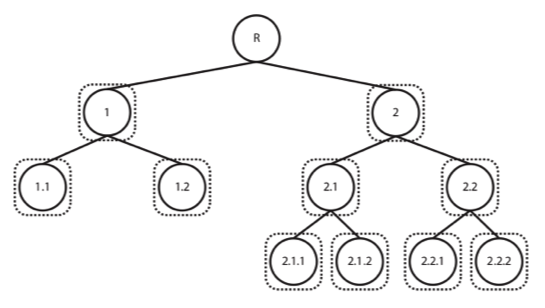
\includegraphics[width=1.0\textwidth]{Figures/hierachical.png}
    \decoRule
    \caption[Hierarchical Classification example]{Hierarchical Classification example (Image credit \cite{Silla2011})}
    \label{fig:hierachical}
\end{figure}

Thus, according to the true path rule, an example that belongs to some class automatically belongs to all its ancestors,
and negative predictions for a given node are propagated to the descendants to
preserve the consistency of the hierarchy. 

Typical examples of hierarchical domains
are protein function prediction and text categorization.
In \cite{Cerri2012} and \cite{Silla2011} two approaches for hierarchical multi-label classification are
described: the local one (top-down) consists of training a hierarchy of classifiers, which are used in a top-down fashion for the classification of new examples; and the global one (one-shot, big-bang), that induces
a unique classifier using all classes of the hierarchy at once and is able to predict just in one step. 

On the other hand, three baseline approaches were identified in \cite{Vens2008}, the two first corresponded to local methods and the last one corresponded
to global methods: Single-label Classification approach (SC), Hierarchical Single-label Classification (HSC) and Hierarchical Multi-label Classification (HMC).
SC trains a binary classifier for each label in the hierarchy considering as
positive examples those labeled with such class and the rest are considered to be
negative. This approach has several drawbacks. 

First, it needs to train one classifier per class (which can be hundreds or thousands). 
Besides, as the hierarchy is not taken into account, it is also possible having inconsistencies. 
Finally, it is very likely having a problem of imbalanced data at lower levels of the hierarchy with only a few positive patterns and too many negative ones \cite{Gibaja2014}.


%----------------------------------------------------------------------------------------

\section{Related Work}

Since the problem faced in this paper is a yearly contest held by the AcousticBrainz project \cite{genretask} 
some several contestants and applications submit their solutions with different approaches and algorithms to tackle this problem.

Submission from previous editions of the task have explored the late fusion of predictions made by classifier models trained for each genre
source individually. In order to predict genres following a taxonomy
of a target source, the proposed solutions applied genre mapping
between taxonomies, either by computing genre co-occurrences on
the intersection of all four training genre datasets \cite{koutinimediaeval}, or by textual
string matching \cite{Murauer2017}.

Schreiber, H \cite{schreiber2018mediaeval} used a CNN network alongside the provided Mel features.

Oramas et al. in \cite{oramas2018mediaeval} propose two different approaches using all the available low level features.

%----------------------------------------------------------------------------------------
 
% Chapter 3

\chapter{Problem Description}

\label{problemdescription}

This section provides an overview of the AcousticBrainz Genre Task
organized as part of the MediaEval 2018 Benchmarking Initiative for
Multimedia Evaluation. 

The task is focused on content-based music
genre recognition using genre annotations from multiple sources
and large-scale music features data available in the AcousticBrainz
database \cite{Porter2015}. 

The goal of this task is to explore how the same music
pieces can be annotated differently by different approaches following different genre taxonomies, and how this should be addressed
by content-based genre recognition systems \cite{Bogdanov2018}. 

%----------------------------------------------------------------------------------------

\section{Data distribution}

Three public available datasets containing genre and subgenre annotations extracted from four different online metadata sources are provided:

\begin{table}[!htb]
    \centering
    \begin{tabular}{l c c c c} 
        \hline
        Dataset & Discogs & Lastfm & Tagtraum \\ [0.5ex] 
        \hline
        Recordings & 904944 & 566710 & 486740 \\ 
        Genres & 15 & 30 & 31 \\
        Subgenres & 300 & 297 & 265 \\
        Genres/track  & 1.37 & 1.14 & 1.13 \\
        Subgenres/track & 1.69 & 1.28 & 1.72 \\
        \hline
    \end{tabular}
    \caption{Overview of the genre distribution}
    \label{table:genredist}
\end{table}

\begin{figure}[!htb]
    \centering
    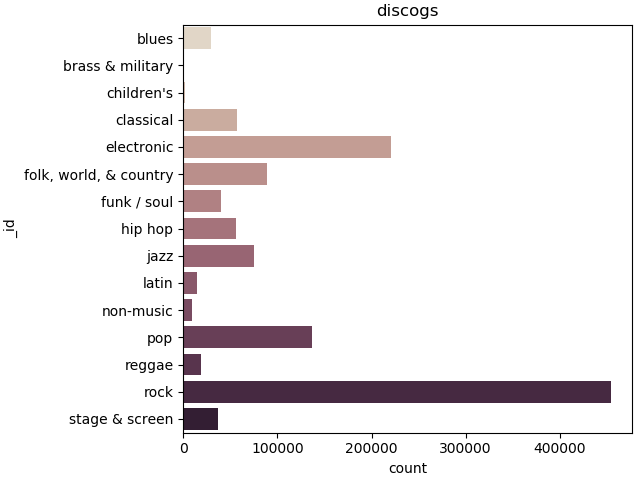
\includegraphics[width=1.0\textwidth]{Figures/discogs_dist.png}
    \decoRule
    \caption[Discogs distribution]{Overview of the Discogs dataset genre distribution}
    \label{fig:discogsdistfig}
\end{figure}
\begin{table}[!htb]
    \centering
    \begin{tabular}{l r} 
        \hline
        Genre & Recordings \\ [0.5ex] 
        \hline
        brass \& military & 1018 \\
        children's & 2267 \\
        non-music & 8825 \\
        latin & 14868 \\
        reggae & 18488 \\
        blues & 29188 \\
        stage \& screen & 37259 \\
        funk / soul & 39621 \\
        hip hop & 56426 \\
        classical & 56643 \\
        jazz & 75539 \\
        folk, world, \& country & 88480 \\
        pop & 136567 \\
        electronic & 220745 \\
        rock & 454272 \\
        \hline
    \end{tabular}
    \caption{Discogs genre distribution}
    \label{table:discogsdist}
\end{table}

\begin{figure}[!htb]
    \centering
    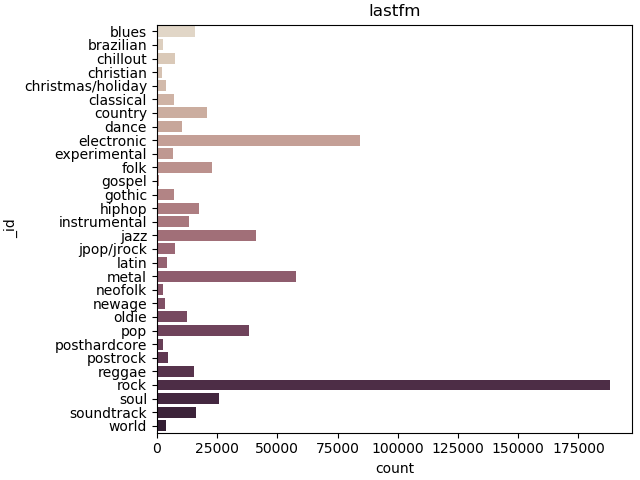
\includegraphics[width=1.0\textwidth]{Figures/lastfm_dist.png}
    \decoRule
    \caption[Lastfm distribution]{Overview of the Lastfm dataset genre distribution}
    \label{fig:lastfmdistfig}
\end{figure}
\begin{table}[!htb]
    \centering
    \begin{tabular}{l r} 
        \hline
        Genre & Recordings \\ [0.5ex] 
        \hline
        gospel & 873  \\
        christian & 1985  \\
        brazilian & 2504  \\
        posthardcore & 2524  \\
        neofolk & 2610  \\
        newage & 3511  \\
        christmas/holiday & 3597  \\
        world & 3819  \\
        latin & 4141  \\
        postrock & 4830  \\
        experimental & 6776  \\
        classical & 7058  \\
        gothic & 7139  \\
        chillout & 7517  \\
        jpop/jrock & 7595  \\
        dance & 10379  \\
        oldie & 12463  \\
        instrumental & 13280  \\
        reggae & 15450  \\
        blues & 15703  \\
        soundtrack & 16370  \\
        hiphop & 17331  \\
        country & 20646  \\
        folk & 22720  \\
        soul & 25673  \\
        pop & 38328  \\
        jazz & 41150  \\
        metal & 57790  \\
        electronic & 84325  \\
        rock & 187955  \\
        \hline
    \end{tabular}
    \caption{Lastfm genre distribution}
    \label{table:lastfmdist}
\end{table}

\begin{figure}[!htb]
    \centering
    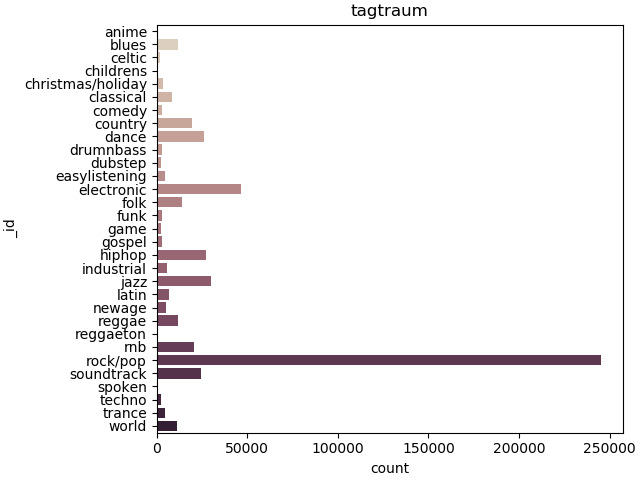
\includegraphics[width=1.0\textwidth]{Figures/tagtraum_dist.png}
    \decoRule
    \caption[Tagtraum distribution]{Overview of the Tagtraum dataset genre distribution}
    \label{fig:tagtraumdistfig}
\end{figure}
\begin{table}[!htb]
    \centering
    \begin{tabular}{l r} 
        \hline
        Genre & Recordings \\ [0.5ex] 
        \hline
        reggaeton & 130 \\
        spoken & 249 \\
        anime & 354 \\
        childrens & 780 \\
        celtic & 1859 \\
        techno & 2045 \\
        game & 2225 \\
        dubstep & 2340 \\
        comedy & 2604 \\
        gospel & 2793 \\
        drumnbass & 2864 \\
        funk & 2953 \\
        christmas/holiday & 3201 \\
        easylistening & 4413 \\
        trance & 4707 \\
        newage & 5286 \\
        industrial & 5809 \\
        latin & 6857 \\
        classical & 8569 \\
        world & 11373 \\
        reggae & 11886 \\
        blues & 11948 \\
        folk & 13697 \\
        country & 19436 \\
        rnb & 20711 \\
        soundtrack & 24476 \\
        dance & 25974 \\
        hiphop & 27038 \\
        jazz & 30096 \\
        electronic & 46292 \\
        rock/pop & 245080 \\
        \hline
    \end{tabular}
    \caption{Tagtraum genre distribution}
    \label{table:tagtraumdist}
\end{table}


%----------------------------------------------------------------------------------------

\section{Music Features}

The dataset provided consists of features precomputed from audio for every music recording. 
The dataset can be downloaded as an archive. 
It contains a JSON\cite{json} file with music features for every RecordingID. 
An example can be seen in \ref{AppendixB}.

All music features are taken from the community-built database AcousticBrainz and were extracted from audio using Essentia, an open-source library for music audio analysis \cite{essentia}. 
They are grouped into categories (low-level, rhythm, and tonal) \cite{essentiafeatures}, \cite{Bogdanov2013}. 
Only statistical characterization of time frames is provided (bag of features), no frame-level data is available.

%----------------------------------------------------------------------------------------

\section{Dataset status}

All three training genre datasets are distributed as CSV files with the following format:

\begin{lstlisting}[caption=CSV Ground Truth]
[RecordingID] [ReleaseGroupID] [genre/subgenre label] ...
\end{lstlisting}

Each line corresponds to one recording (a music track or song) and contains all its ground-truth genre and subgenre labels. 

RecordingID is the MusicBrainz identifier of the particular recording. 
To distinguish between genre and subgenre labels, subgenre strings are compound and contain --- as a separator between a parent genre and an actual subgenre name. 
For example, rock, electronic, jazz and hip hop are genres, 
while electronic---ambient, rock---singersongwriter and jazz---latinjazz are subgenres.

ReleaseGroupID is a MusicBrainz identifier of a release group (an album, single, or compilation) that it belongs to. 

%----------------------------------------------------------------------------------------

\section{Processed data}

To avoid having unbalanced data on each of the labels several adjustment methods are used.

\begin{itemize}
    \item Pruning: Simply removing the label and all its recordings that are under a certain threshold value.
    \item Thresholding: Limiting the number of documents that exceed a certain upper bound to that limit.
    \item Artificial balancing: Creating fake examples of underrepresented genres using statistical methods to balance the dataset. See more in \ref{initialapproach}. 
\end{itemize}

%----------------------------------------------------------------------------------------


% Chapter 4

\chapter{Approach}

\label{approach}
The following sections will deeply explore and describe the insights of the project and the development process and the decisions taken with the reasons behind it. 
These sections imply a higher technical language and background filled with several domain-specific vocabularies.

%----------------------------------------------------------------------------------------

\section{Environment Architecture}
In this section, the different methodologies, programming tools and abstractions used during the project may be discussed and how the code is built around them.

\subsection{Python}
Python is a multi-purpose open-source programming language focused on the quick prototyping. Using a really simple language syntax makes any inexperienced programmer be able to comprehend and create simple scripts. 
Since there is no compilation, the debugging step is especially fast and repeating the cycle of editing and running is reduced in time\cite{pythonabout}.
Given the multiple open-source libraries and frameworks available for Machine Learning and Artificial Intelligence, Python is a great and suitable option to develop a project with the needed characteristics.
Some of the mentioned libraries that will be used along with the project:

\begin{itemize}
    \item NumPy: package for scientific computing with Python \cite{numpy}.
    \item pandas: library providing high-performance, easy-to-use data structures, and data analysis tools for the Python programming language \cite{pandas}.
    \item scikit-learn: Machine Learning module providing efficient tools for data mining and data analysis \cite{scikit}.
    \item Matplotlib  2D plotting library \cite{matplotlib}.
    \item seaborn: data visualization library. It provides a high-level interface for drawing attractive and informative statistical graphics \cite{seaborn}.
\end{itemize}


\subsection{MongoDB}
MongoDB is a general-purpose, document-based, distributed database \cite{mongo}.
With a powerful query syntax and language is pretty straightforward to build complex databases and retrieve the desired records with ease.
Since it is based on the JSON\cite{json} standard it allows creating complex records using arrays, nested properties, and key-value pairs.
Despite the traditional relation Databases using the SQL standards, MongoDB is a nonrelational database relaying on the NoSQL (Not Only SQL) syntax and instead of using tables and rows as in relational databases, MongoDB is built around collections and documents.

Given the previously described problem, MongoDB is a perfect and suitable option to depend on for storing and retrieving the music datasets available. With just some simple commands it easy to obtain the desired data, a chunk of it or more complex subsets that need to fit special conditions to better approximate the model standards.

\subsection{Tensorflow}
Tensorflow is an open-source mathematical computing library used as a backend for heavily expensive operations.
It offers different levels of abstractions so it can work easily coupled with different libraries that rely on heavy calculations and operations with matrixes or tensors.

It provides a collection of workflows to develop and train models using different programming languages so even though it was publicly released in 2015 it is the preferred option to build Machine Learning models as Artificial Neural Networks, the main topic of this thesis \cite{tensorflow}.

\subsection{Keras}
Keras is a high-level neural networks API, capable of running on top of TensorFlow. 
It is focused on enabling fast experimentation and prototyping using a friendly user-interface API, modularity, and extensibility. 

Supports most of the most common known Artifical Neural Networks types such a Deep Neural Networks, Convolutional Neural Networks, and Recurrent Neural Networks or any combination of the previously mentioned ones. 
Nonetheless, implementing your custom layers and metrics is easy in case the basic framework does not suit your needs.

Relying on TensorFlow as the mathematical background allows running seamlessly on both the CPU and the GPU thus heavy models with extensive training phases can be easily computed across different machines alleviating the load from one system to multiple ones.

\newpage
%----------------------------------------------------------------------------------------

\section{Basic stack}
The following section briefly explains how the components already mentioned are connected and used during the whole project.
The project consists of several scripts that handle each one of the individual tasks, only the main ones will be discussed in this paper:

\begin{itemize}
    \item Database Warmer: This script takes the provided CSV files to process them and creates a ready-to-use document for each of the songs to be inserted into the MongoDB Database. This is a one-use-only script that is crucial to be able to retrieve the desired songs afterward.
    \begin{figure}[th]
        \centering
        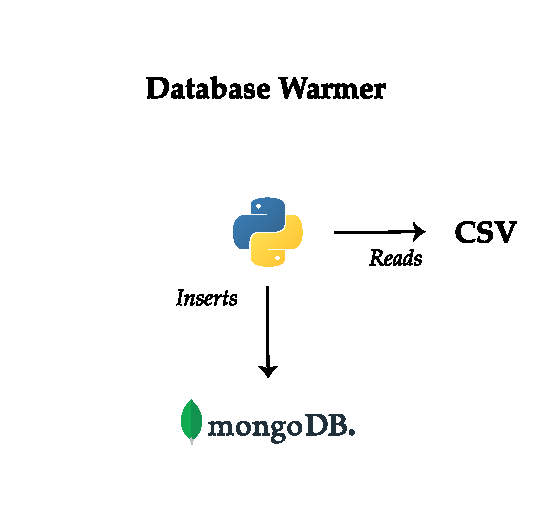
\includegraphics{Figures/DatabaseWarmer}
        \decoRule
        \caption[Database Warmer Script]{Diagram detailing the database warming process}
        \label{fig:Database Warmer Script}
    \end{figure}


    Here is an example of one of the documents inserted:
    \begin{lstlisting}[caption=Song JSON document]
{
    "_id": "5cadfc2f4fac9e1e50b0ad5a",
    "mbid": "1a00a335-fead-46ec-8d4f-06e8341291ea",
    "release": "0f2ccf4d-d242-3c23-a419-ea548af51df3",
    "genres": [
        {
        "name": "electronic",
        "genres": [
            {
            "name": "ambient",
            "genres": []
            },
            {
            "name": "trance",
            "genres": []
            }
        ]
        }
    ]
}
    \end{lstlisting}

    
    \item Main Script This script is in charge of the entire process and stages model related:
    \begin{enumerate}
        
        \item Train: This is the base stage of the process, the script connects with the Database and retrieves the dataset to be used as training, loads and builds the model in Keras and proceeds to train the model using TensorFlow, once the training process is finished the trained model is stored in the disk and the results are evaluated in the test stage.
        \begin{figure}[th]
            \centering
            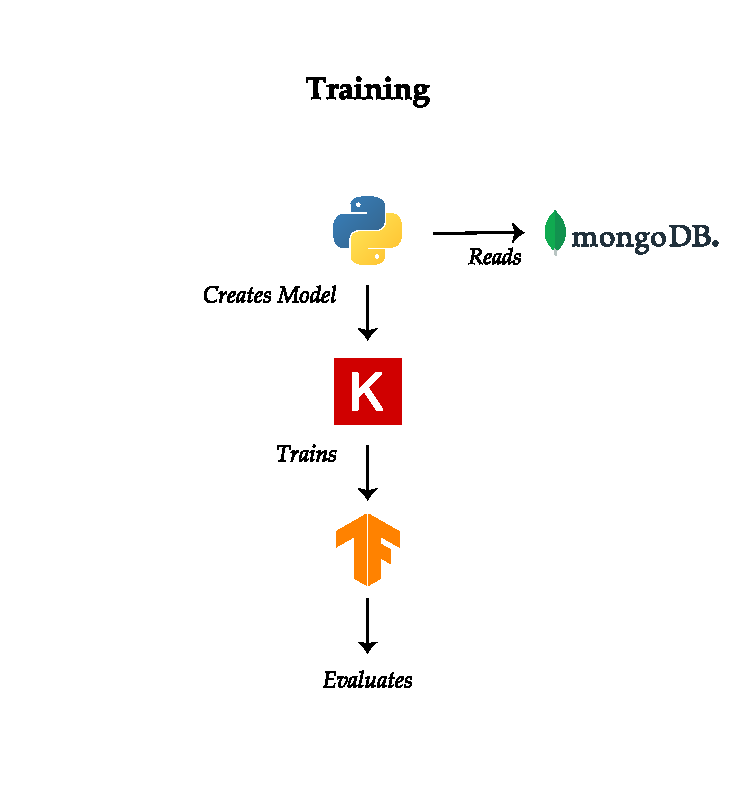
\includegraphics{Figures/TrainStage}
            \decoRule
            \caption[Train Stage]{Diagram detailing the training stage}
            \label{fig:Train Stage}
        \end{figure}
        
        \item Test: Once the model is trained its performance should be evaluated with data apart from the examples used in the training, to avoid the overfitting. For this case of the matter, the new examples are fed to the trained model and its outputs predicted and checked against its known outputs.
        \begin{figure}[th]
            \centering
            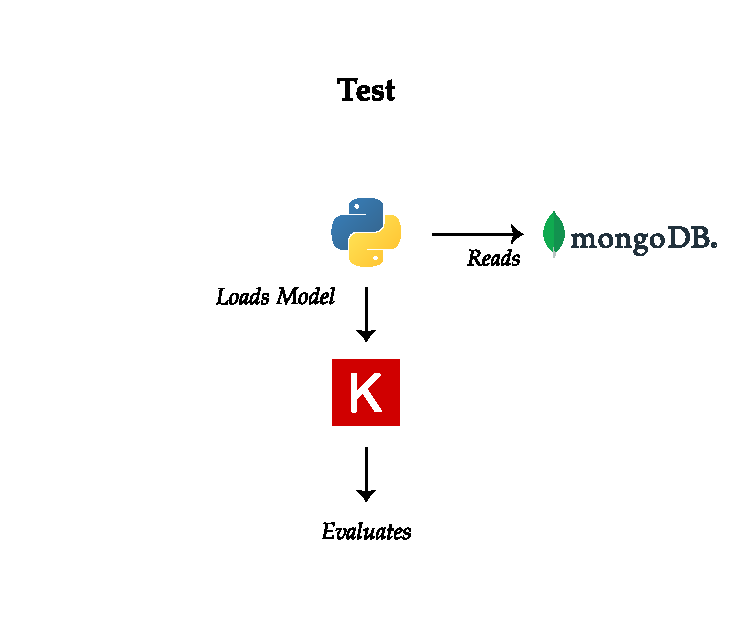
\includegraphics{Figures/TestStage}
            \decoRule
            \caption[Test Stage]{Diagram detailing the test stage}
            \label{fig:Test Stage}
        \end{figure}
        
        \item Predict: This phase is obtained once the proper model with the best outcome is built and trained. It properly labels new and unknown songs.
        \begin{figure}[th]
            \centering
            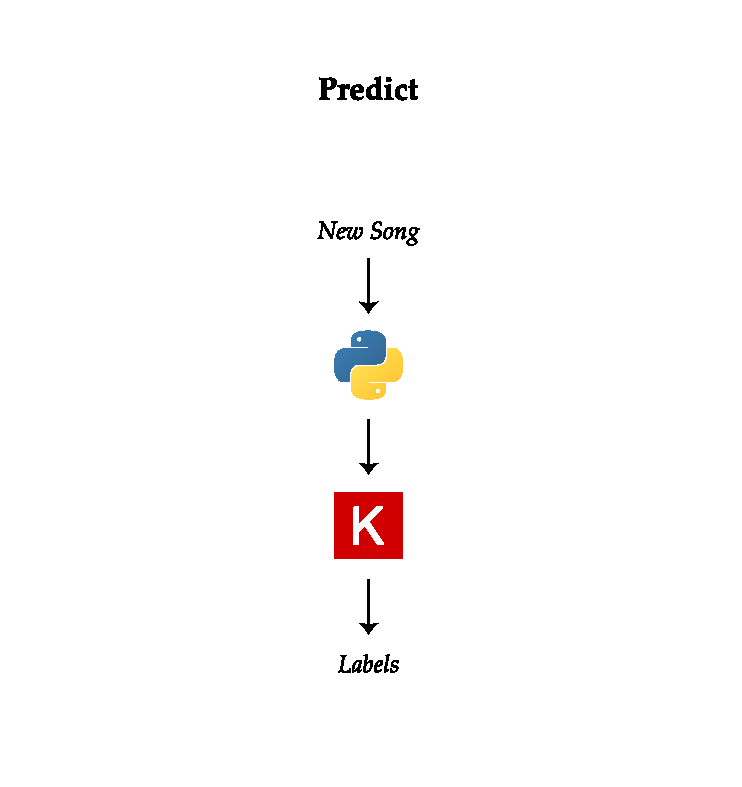
\includegraphics{Figures/PredictStage}
            \decoRule
            \caption[Predict stage]{Diagram detailing predict stage}
            \label{fig:Predict Stage}
        \end{figure}

    \end{enumerate}

\end{itemize}

\newpage
%----------------------------------------------------------------------------------------

\section{Initial approach}

In this section, the initial model and its next iterations will be discussed and explained along with the different design options taken during the process.

As mentioned in previous sections this thesis constitutes a Multi-Label classification problem so using the related work as a starting point there are two main architectures:

\subsection{Multi-Label single output}
This method produces a single output for each of the songs fed and it has a neuron in the last layer for every genre $N$ available. Each one of those \(N\) neurons will hold the probability of that genre being present given an example \(x\) using the following expression:
$$ P(\hat{y} = i | x) \forall i \in N$$
This produces a probability vector $\hat{Y}$ that is pruned using a threshold value to obtain the highest probability genres.

The target $Y$ is obtained using the following mapping
$$
\bar{y_i} =
\begin{cases} 
    1 & \text{if } y_j \in S\\
    0 & \text{if } y_j \notin S\\
\end{cases}
\forall j \in N
$$

So given an example with the following genres:

$$ y  = [ Pop, Rock ]$$

And the available genres in the set:
$$ S  = [Jazz, Pop, Rock, Soul]$$
Will produce the output:
$$ \bar{y}  = [0, 1, 1, 0]$$

Then $Y$  is constructed as follows
$$ Y = [y_0, y_1, y_2 ... y_m]^T$$
Where $m$ is the number of examples to feed to the network.

To avoid overfitting it is important to provide a balanced dataset $Y$ otherwise the Network may suffer from overfitting.
To do so some artificial balancing methods such as SMOTE\cite{Chawla2002} \cite{Blagus2013} may be used

In general:
$$ |y^i| \approx \frac{m}{N}   \forall i \in N $$
being:
$$ m > N $$
And:
$$ \sum_{i=1}^{N} |y^i| \approx m $$

\subsection{Binary-Label multiple output}
This method differs from the previous one as several classifiers $c_i$ are trained for each of the available genres $N$. Each one of the classifiers will provide the statistical probability of a song being of that genre.
This creates an ensemble of classifiers $C$ :
$$ C = \{c_1, c_2, c_3 ... c_N\} $$ 

So given a predict function  $f(x, c)$, an example $x$ and a classifier $c_i$ 

$$ f(x, c_i) =  P(\hat{y_i} = i | x) \forall i \in N $$

Therefore the complete predicted vector $\hat{y}$ is defined as follows:
$$ \hat{y} = [ \hat{y_1}, \hat{y_2}, \hat{y_3} ... \hat{y_N} ] $$

In this case, the target matrix \(Y\) constitutes a column vector obtained using the following mapping:
$$ {y_i} =
\begin{cases}
    1 & \text{if } y_i \in S\\
    0 & \text{if } y_i \notin S\\
\end{cases}
$$
Therefore:
$$ Y = [y_0, y_1, y_2 ... y_m]^T $$
Where $m$ is the number of examples.

Given a binary classifier, the important point here is to have a similar number of positives examples $y^+$ as negative ones $y^-$ so:
$$ |y^+|  \approx \frac{m}{2} $$
$$ |y^-|  \approx \frac{m}{2} $$
$$ |y^+| + |y^-| \approx m $$

For example, for the classifier $c_{Pop}$ and the song :
$$ y_t  = [ Pop, Rock ] $$
Will produce the output:
$$ \bar{y_t}  = 1 $$

On the contrary, the song:
$$ y_k  = [ Jazz, Soul ] $$
Will produce the output:
$$ \bar{y_k}  = 0 $$

%----------------------------------------------------------------------------------------

\section{Feature selection}
This section is purely dedicated to explain of the training matrix $X$ is built.
This matrix is used regardless of the network architecture and should work in any iteration of the model

The main important aspect to weight in is the number of single features to choose as it will affect the number of neurons in the input layer.

To see all the available features of the provided dataset refer to Appendix \ref{AppendixA}

According to the base material the most promising features to elaborate a genre classifier model are the MFCC \cite{Jensen2006} \cite{Li2011}.

The mentioned features are stacked into a vector $x_i$ and normalized to avoid overweighting the rest of the features 
Then the input matrix is built using:

$$X = [x_1, x_2, x_3, ... x_m]$$

%----------------------------------------------------------------------------------------

\section{Data processing}

To avoid having a heavy model on the input and obtain the most prominent features a PCA is applied thus reducing the number of features in the input \cite{pca} \cite{Minka2001}: 
Given $X$ belonging to $\mathbb{R}^m$ the idea is finding a reduction of $ X' \in \mathbb{R}^n$ where $n < m$ that explains a certain percentage of the variance of the original matrix $X$.

When doing predicitions and tests it is important to reduce the new matrixes to prune the number of components to $n$. 

%----------------------------------------------------------------------------------------

\section{ANN architecture}
The architectures for both approaches are shown below. 
Both models are constructed using a Feed-forward MLP consisting of several layers
%----------------------------------------------------------------------------------------

\section{Training}

%----------------------------------------------------------------------------------------

\section{Validation}
To avoid overfitting and reaching $100\%$ accuracy in the training set and underperform in the test set a validation set is constructed from the training one and fed to the model too.
After each of the epochs in completed the network evaluates its performance against the validation set , that is not used for training and adjusts the weights accordignly in case of overfitting.

We get that

$$X = X^{Train} \cup X^{Validation}$$
$$X^{Train} \cap X^{Validation} =  \emptyset $$

Between each layer an addtional Dropout layer is included to add random uniform noise and obtain a better performance \cite{Srivastava2014}.

On top of that to validate the overall performance a k-fold cross validation method is used \cite{Rodriguez2010}.
This method divides the entire dataset into $k$ random independant sets and trains the model $k$ times using $k - 1$ sets as training and the remaining one as test
To calculate the accuracy we can get use a simple mean from all the models accuracy

$$acc_{m} = \frac{1}{k}\sum_{i=1}^{k} acc_{m_{i}}$$


%----------------------------------------------------------------------------------------

\section{Test}

\cite{Flach2015}
\cite{Davis2006}

%----------------------------------------------------------------------------------------

\section{Prediction}

New song comes
    Audio -> extract features
    Features

    PCA


    Prediction

    Labeling

%----------------------------------------------------------------------------------------

 
%% Chapter 4

\chapter{Conclusions}

\label{conclusions}
%----------------------------------------------------------------------------------------
As seen in the \ref{test stage} the performance obtained by all the proposed models is not positive enough to deploy these models in a production environment.

During this whole thesis development project, several approaches and iterations have been explored to improve the efficiency of the overall model with unsatisfactory outputs.

Based on the state of the art \ref{stateofart} analysis different papers seems to reach poor performance with disappointing results.

It can be concluded that song deep features combined with MLP models are not a suitable option and approach to label musical pieces. 

As already mentioned labeling genres is a complex and ongoing task that still needs development and further investigation, really subtle details can determine whether a song belongs to a genre or another. This task is even complicated for humans too that sometimes can not agree to which genre a song fits to. 

When does a song be different enough to constitute a genre itself?

Is it a sub-genre or a completely new one?

\section{Achieved goals}
The primary goal of creating an Artificial Neural Network capable of labeling songs has been achieved.

This Network is able to label with more than one genre to a song constituting a Multi-label Multi-Class classification problem.

The model can label genres hierarchically creating several classifiers recursively complying with the established genre ontology.

\section{Pending goals}
Improve the model performance and surpass the outcome defined in the state of the art for the same problem.

\section{Further work}
To properly label song that is the main task of this paper some different alternatives can be chosen:

\begin{itemize}
	\item Use different architectures. Play with different MLP models and architectures. Using a Convolutional Neural Network along with the song spectrogram is a promising task that can produce better conclusions.
	\item Use different features. Combine and test different song features. Due to the limitations of the provided dataset some extra features that might have been useful could not be used.
	\item Explore different algorithms. Maybe the MLP is not a suitable solution to tackle the genre classification problem. Using alternatives could improve the performance like Support Vector Machines o Nearest Neighbors to name a few.
	\item Combining different ML techniques might improve the results, appointing the previous point, the use of several algorithms for small and highly coupled tasks can lead to superior results.
\end{itemize}
 

%----------------------------------------------------------------------------------------
%	THESIS CONTENT - APPENDICES
%----------------------------------------------------------------------------------------

\appendix % Cue to tell LaTeX that the following "chapters" are Appendices

% Include the appendices of the thesis as separate files from the Appendices folder
% Uncomment the lines as you write the Appendices

% Appendix A

\chapter{Song Deep Features}

\label{AppendixA}

\begin{lstlisting}[caption=Song Deep Features]

\end{lstlisting}



%% Appendix B

\chapter{Song Deep Features}

\label{AppendixB}

All song deep features can be viewed from this example

\url{https://acousticbrainz.org/a3b8950a-d1f8-49b9-b88f-89f38726f332/low-level/view?n=0}

All the features and musis descriptors are explained in \cite{essentiafeatures}



%% Appendix C

\chapter{Song Deep Features}

\label{AppendixB}

All song deep features can be viewed from this example

\url{https://acousticbrainz.org/a3b8950a-d1f8-49b9-b88f-89f38726f332/low-level/view?n=0}

All the features and music descriptors are explained in \cite{essentiafeatures}




%----------------------------------------------------------------------------------------
%	BIBLIOGRAPHY
%----------------------------------------------------------------------------------------

\printbibliography[heading=bibintoc]

%----------------------------------------------------------------------------------------

\end{document}  
